\chapter{Transistors}

%\section{Chapter Overview}
A transistor is a semiconductor device used to amplify or switch electrical signals and power.  It is a component with (at least) three terminals. A voltage or current applied to one of the  terminals controls the current through another pair of terminals. Because the controlled (output) power can be higher than the controlling (input) power, a transistor can amplify a signal.\\
%We will discuss the bipolar junction transistor (BJT) and two transistors based on the field-effect, namely the junction FET and the Metal-Oxide-Semiconductor Field Effect transistor (MOSFET).
We will discuss the two most prevalent transistors: the Bipolar Junction Transistor (BJT) and the Metal-Oxide-Semiconductor Field Effect transistor (MOSFET).
\section{Bipolar Junction Transistor}
\label{sec:bipolar_junction}
A bipolar junction transistor (BJT) is formed by placing a n-type semiconductor between two p-type semiconductors (pnp) - or vice versa (npn), as shown in figure \ref{fig:bjt1}. In the case of the pnp transistor, the heavily doped $p^+$-region is called the \emph{emitter} (E). The narrow central $n$-region is the \emph{base} (B). Its width is small compared with the diffusion length of the minority carriers. The lightly doped $p$-region is the \emph{collector} (C). Figure \ref{fig:bjt1} also shows the circuit symbols for the two BJT transistors, together with the conventional directions for voltages and currents.\\
We will discuss the pnp-transistor in some detail; the reasoning for the npn-transistor is similar and left as an exercise.

\begin{figure}[h!]
\centering
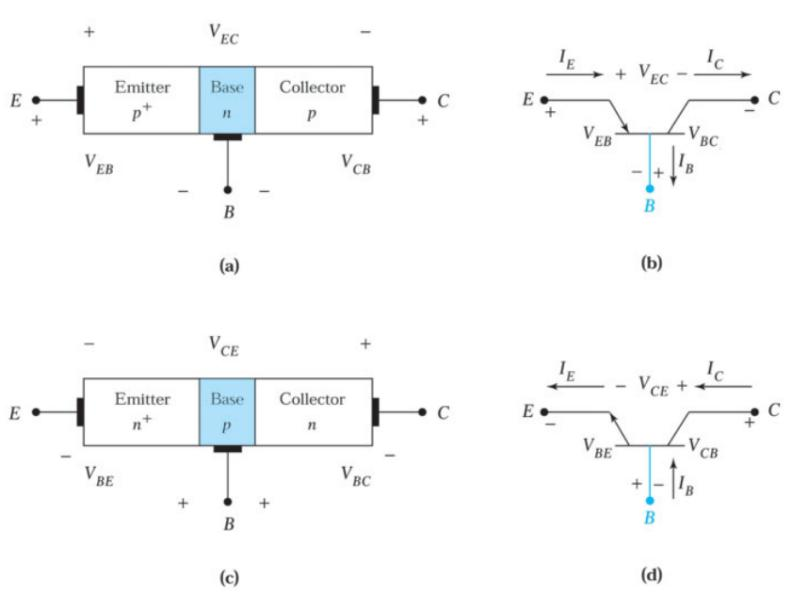
\includegraphics[width=12cm]{figures/ch01/bjt1.jpg}
\caption{(a) Idealized one-dimensional schematic of a p-n-p bipolar transistor and (b) its circuit symbol. (c) Idealized one- dimensional schematic of an n-p-n bipolar transistor and (d) its circuit symbol.} 
\label{fig:bjt1}
\end{figure}

\subsection{Operation in Active Mode}
First consider the pnp-transitor with the three terminals (emitter, base and collector) connected to ground as in figure \ref{fig:bjt2} (a). Under these circumstances we can construct the charge profile like we did for the pn-junction. Notice that the space-charge regions at both junctions extend deeper in the lower doped regions (base in E-B junction, collector in B-C junction).

\begin{figure}[h!]
\centering
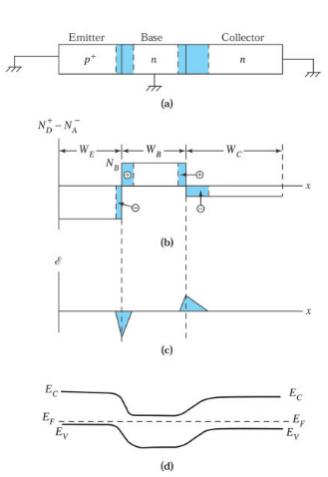
\includegraphics[width=8cm]{figures/ch01/bjt2.jpg}
\caption{(a) pnp transistor with all leads grounded (b) Charge profile in equilibrium (c) Electric field (d) Energy band diagram.} 
\label{fig:bjt2}
\end{figure}
As for the pn-junction, the electric field that emerges in the space-charge region is such that it in equilibrium with the diffusion current due to the concentration gradients at the junctions. Figure \ref{fig:bjt2}(d) shows the band diagram in equilibrium. Since there is no current, the Fermi-level $E_F$ is constant in the three regions.\\
We will polarize the transistor in the so-called active mode. This is the most commonly used mode in practice. We do this by applying a positive voltage $V_{EB} > 0$ between emitter and base, and a negative voltage $V_{CB} < 0$ between collector and base. The pn-junction between emitter and base is thus forward-biased, while the junction between collector and base is reversed biased.\\
Since we apply a positive voltage to the emitter and a negative voltage to the collector (while keeping the base grounded; this is a \emph{common-base} configuration), we lower the energy bands in the emitter and raise them in the collector (just as in the pn-junction) - see figure \ref{fig:bjt3}(d). As a consequence, the potential barrier between emitter and base is lowered so majority carriers of the emitter side (i.e. holes) can diffuse through the space-charge region to the base. If the base would be a lot larger than the diffusion length, almost all injected holes would recombine with electrons in the base and generate a base current, just like in an ordinary pn-junction. However, since the base is small, most injected holes do not recombine but diffuse into the space-charge region between base and collector. There they are swept by the electrical field to the collector. As a consequence, most holes leaving the emitter end up in the collector. This phenomenon is called the \emph{transistor action}. It is important to realize that the collector current depends on the emitter current and thus on the height of the emitter-base barrier and $V_{EB}$, but not on the base-collector voltage $V_{CB}$ (as long as the base-collector junction is reversed biased).

\begin{figure}[h!]
\centering
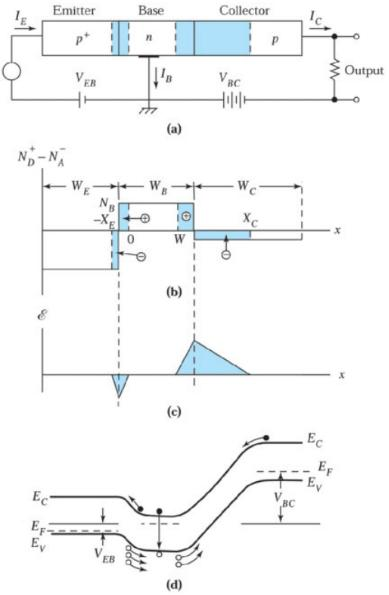
\includegraphics[width=8cm]{figures/ch01/bjt3.jpg}
\caption{pnp transistor in active mode} 
\label{fig:bjt3}
\end{figure}

\subsection{Currents in Active Mode}
For each terminal, we can identify the carrier flows that contribute to the currents $I_E$, $I_C$ and $I_B$.
\begin{enumerate}
    \item At the emitter:
    \begin{itemize}
        \item a hole current from emitter to the base $I_{Ep}$
        \item an electron flow from base to emitter $I_{En}$
    \end{itemize}
    Thus $I_E = I_{Ep} + I_{En}$
    \item At the base:
    \begin{itemize}
        \item a current $I_{BB}$ due to recombination of injected holes with electrons (which have to be resupplied by the battery). This current equals the difference between $I_{Ep}$ and $I_{Cp}$: $I_{BB} = I_{Ep} - I_{Cp}$
        \item an electron flow from base to emitter $I_{En}$
        \item an electron flow from collector to base: $I_{Cn}$ (i.e. the leakage current from the reversed biased B-C junction)
    \end{itemize}
    Thus $I_B = I_{En} + (I_{Ep} - I_{Cp}) - I_{Cn}$
    \item At the collector:
    \begin{itemize}
        \item a current $I_{Cp}$ that is what remains of $I_{Ep}$ after transition through the base.
        \item an electron flow from collector to base through the reversed biased B-C junction: $I_{Cn}$ 
    \end{itemize}
    Thus $I_C = I_{Cp} + I_{Cn}$
\end{enumerate}
These currents are represented in figure \ref{fig:bjt4}. As the figure implies, $I_{Ep}$ is the major current in the device.

\begin{figure}[h!]
\centering
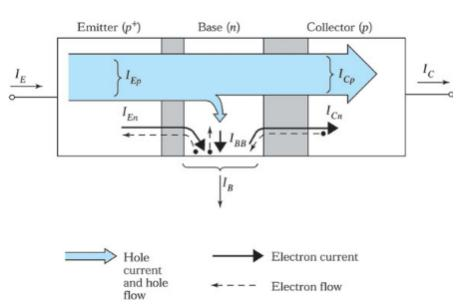
\includegraphics[width=11cm]{figures/ch01/bjt4.jpg}
\caption{Currents in active mode} 
\label{fig:bjt4}
\end{figure}

We characterize the transistor by the \emph{common-base current gain} $\alpha_0$, which is the ratio between $I_{Cp}$ and the emitter current:
$$
\alpha_0 \equiv \frac{I_{CP}}{I_E}
$$
We can rewrite this as:
$$
\alpha_0 = \frac{I_{Cp}}{I_{En} + I_{Ep}} = \Big(\frac{I_{Ep}}{I_{En} + I_{Ep}}\Big)  \Big(\frac{I_{Cp}}{I_{Ep}}\Big) = \alpha_T \; \gamma
$$
with $\alpha_T $ the \emph{base transfer factor} and $\gamma$ the \emph{emitter efficiency}. For proper operation, we require that $I_{Ep} \gg I_{En}$, thus that $\alpha_T \approx 1$. This can be accomplished by requiring that the emitter doping level be much greater than that of the base. The factor $\gamma$ can be increased by decreasing the length of the base.\\
We can rewrite the collector current $I_C$ as:
\begin{equation}
    \begin{split}
        I_C &= I_{Cp} + I_{Cn} = \alpha_T I_{Ep} = \alpha_0 I_E + I_{Cn} \\
            &= \alpha_0 I_E + I_{CB0} \\
    \end{split}
    \label{eq:bjt1}
\end{equation}
where $I_{CB0} $ is the leakage current between collector and base with the emitter-base junction open. This expresses that the collector current is a fraction ($0 < \alpha_0 < 1$) of the emitter current, plus a leakage current.

\subsection{Carrier distribution in Active Mode}
In order to compute the different currents, we first need to determine the carrier distribution in each region. We will assume the following:
\begin{enumerate}
    \item Uniform doping in each region
    \item No hole drift current in base
    \item Collector saturation current is negligible
    \item Only low-level injection
    \item No generation-recombination in the depletion zone
    \item No series resistance in the device
\end{enumerate}

We will assume that the $x=0$ corresponds to the end of the emitter-base depletion zone, and $x=W$ to the start of the base-collector depletion zone. Starting from the continuity equation for minority carriers in the base region:
$$
\frac{dp_n}{dt} = - \frac{(p_n-p_{n0})}{t_p} - \frac{1}{q} \frac{d J_p}{dx} + g \text{ with }  J_p = q \mu_p p E + q D_p \frac{dp_n}{dx}
$$
If we assume steady-state, no electric field and no other generation mechanisms, the equation reduces to:
$$
D_p \frac{d^2 p_n}{dx^2} = \frac{(p_n-p_{n0})}{t_p}
$$
This equation has as general solution
$$
p_n(x) = p_{n0} + C_1  \; e^{x/L_p} + C_2 \;  e^{-x/L_p}
$$
with $L_p = \sqrt{D_p t_p}$ the so-called \emph{diffusion length} of the holes in the n-type semiconductor. Constants $C_1$ and $C_2$ can be determined by the boundary conditions:
\begin{itemize}
    \item $p_n(0) = p_{n0} \;  e^{qV_{EB}/kT}$ because this the standard concentration at the boundary of the depletion region, as in equation \ref{eq:density_junction} of chapter \ref{ch:pnjunction},
    \item $p_n(W) = 0$ because all holes at $x=W$ will be swept through the base-collector space-charge region by the induced electric field.
\end{itemize}
Solving for $C_1$ and $C_2$ leads to a rather complex distribution. However, if $W/L_p \ll 1$ we can simplify and obtain:
$$
p_n(x) = p_{n0}\; e^{qV_{EB}/kT} \; \Big(1 - \frac{x}{W} \Big)
$$
The minority carrier concentration decreases thus linearly in the base. In a similar manner, we can find an expression for the minority carriers (electrons) in emitter and collector. The results are:
\begin{equation}
    \begin{split}
        n_E(x) &= n_{E0} + n_{E0} (e^{qV_{EB}/kT} - 1) e^{(x+x_E)/L_E}\\
        n_C(x) &= n_{C0} - n_{C0} e^{(x-x_C)/L_C}
    \end{split}
\end{equation}
These distributions are also represented in figure \ref{fig:bjt5}. Once the carrier concentrations are known, the currents are easily computed as they are proportional to the concentration gradient:
\begin{itemize}
    \item $I_{Ep} = A \Big(-q D_p \frac{dp_n}{dx}|_{x=0}\Big) = \frac{qAD_p \; p_{n0}}{W} e^{qV_{EB}/kT}$
    \item $I_{En} = A \Big(-q D_E \frac{dn_E}{dx}|_{x=-x_E}\Big) = \frac{qAD_E \; n_{E0}}{L_E} (e^{qV_{EB}/kT}-1)$
    \item \ldots
\end{itemize}
By combining these results, we obtain expressions for the three terminal currents:
\begin{itemize}
    \item $I_E = a_{11} (e^{qV_{EB}/kT} - 1) + a_{12}$
    \item $I_C = a_{12} (e^{qV_{EB}/kT} - 1) + a_{22}$
    \item $I_B = I_E - I_C$
\end{itemize}
where all the $a_{ij}$ depend on the transistor characteristics like doping concentrations and dimensions.
\begin{figure}[h!]
\centering
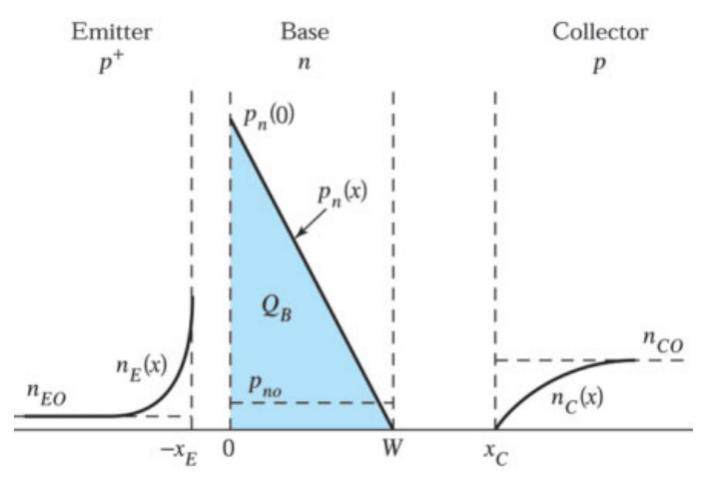
\includegraphics[width=10cm]{figures/ch01/bjt5.jpg}
\caption{Minority carrier distribution in active mode} 
\label{fig:bjt5}
\end{figure}

\subsection{Modes of Operation and Ebers-Moll Equations}
\label{sec:modes_of_operation}
Based on the signs of $V_{EB}$ and $V_{CB}$, we can distinguish $4$ different modes of operation. We already studied the case where $V_{EB} > 0$ and $V_{CB} < 0$, namely the active mode. The other modes are represented in figure \ref{fig:bjt_modes}, together with the minority carrier distribution in emitter, base and collector.
\begin{figure}[h!]
\centering
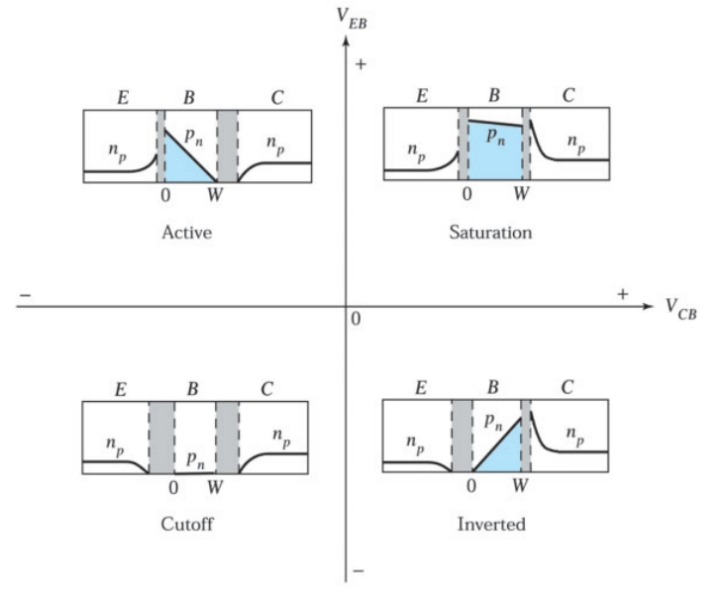
\includegraphics[width=12cm]{figures/ch01/bjt_modes.jpg}
\caption{Modes of operation} 
\label{fig:bjt_modes}
\end{figure}
In saturation mode, both junctions are forward biased. The minority-carrier distribution at the edge of each depletion region is not zero, as in the active mode. Small biasing voltages lead to a large output current. The transistor acts a closed switch.\\
In cuttoff mode, both junctions are reversed biased. Only a small current will flow. The transistor is an open switch.\\
In inverted mode, emitter and collector are reversed. The behavior is however not exactly like in the active mode, because the doping levels in emitter and collector are different.\\
All these modes can be analyzed in a similar way as we have done for the active mode. This analysis leads to the \emph{Ebers-Moll equations} which are used to model the BJT in simulators like SPICE.\\
\textbf{TODO: Add Ebers-Moll equations and equivalent circuits}

\subsection{Common-Emitter configuration}
Up until now, we have kept the base at a fixed voltage. However, the most common use of the bipolar transistor is with the emitter at a fixed voltage as in figure \ref{fig:bjt6}(a). This configuration has $V_{EB}$ and $I_B$ as inputs, and $I_C$ and $V_{EC}$ as outputs.\\
We can express $I_C$ as function of $I_{B}$ by substituting $I_E = I_B + I_C$ in equation \ref{eq:bjt1}:
$$
I_C = \alpha_0 (I_B + I_C) + I_{CBO}
$$
Solving for $I_C$ gives:
\begin{equation}
    \begin{split}
        I_C &= \frac{\alpha_0}{1-\alpha_0} I_B + \frac{I_{CB0}}{1 - \alpha_0}\\
            &= \beta_0 I_B + I_{CE0}
        \label{eq:bjt2}
    \end{split}
\end{equation}
with $\beta_0 = \frac{\alpha_0}{1-\alpha_0}$ the \emph{common-emitter current gain} and $I_{CE0} = \frac{I_{CB0}}{1-\alpha_0}$ the collector-emitter leakage current. This current is always present, even if $I_B=0$ and thus makes the bipolar transistor a very bad switch because it will leak current when closed.\\
In the previous, common-base configuration, and with $\alpha_0 \approx 1$, a change in emitter current $I_E$ produces a changes of approximately the same amount in the collector current $I_C$ and a much smaller change in the base current (factor of $1-\alpha_0$). To achieve current amplification, the change is initiated in the base current rather than in the emitter current. This causes the collector current to change by a factor of $\frac{\alpha_0}{1 - \alpha_0} = \beta_0$.\\
When $\alpha_0$ is close to one, $\beta_0$ becomes very large. This is a good thing because it allows us to amplify the base current $I_B$. However, $\beta_0$ can change a lot from transistor to transistor. This is why we will explore polarisation techniques that mitigate the variability of $\beta_0$.


\begin{figure}[h!]
\centering
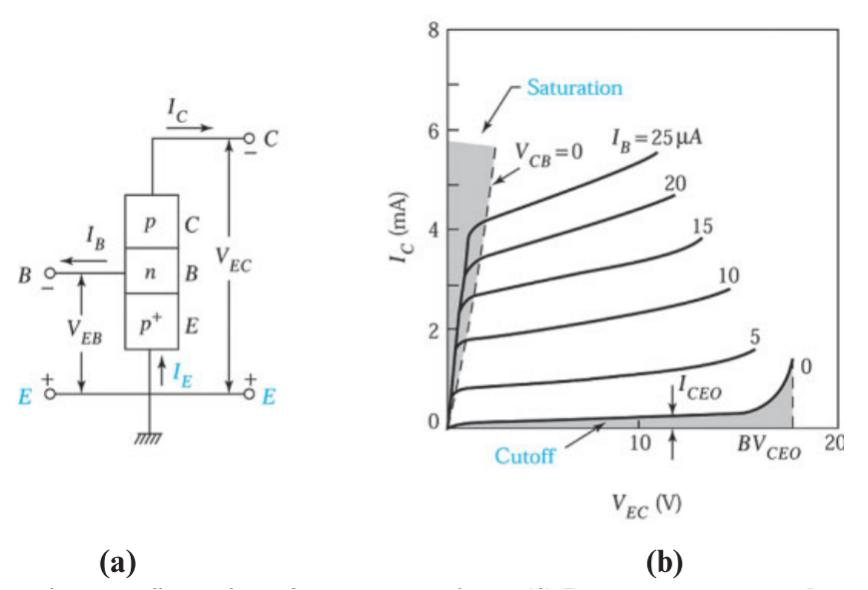
\includegraphics[width=10cm]{figures/ch01/bjt6.jpg}
\caption{BJT in common-emitter configuration (a) and I-V characteristic (b)} 
\label{fig:bjt6}
\end{figure}

The defining I-V characteristic of a common-emitter configuration is shown in \ref{fig:bjt6}(b). If $V_{EC}$ is too low, $V_{CB}$ is positive and the base-collector junction is not reversed biased. The transistor in saturation mode. Thus $V_{EC}$ must be higher than some threshold to put the transistor in the active mode. This value is called $V_{EC, Sat}$ and is about $0.2$ V.\\
When $V_{EC} > V_{EC, Sat}$, we can say based on equation \ref{eq:bjt2} that $I_C \approx \beta_0 I_B$ and hence independent of $V_{EC}$. This is the ideal behavior, because we now control output current $I_C$ with input current $I_B$ and not with the output voltage $V_{EB}$. However, as can be seen from the figure, the I-V characteristics are not entirely flat and thus still depend on $V_{EB}$. This is due to the \emph{Early-effect} and will be addressed in the next section.\\
If $V_{EB}$ is lower than $0.6$ V, the emitter-base junction is not forward biased and $I_B$ is very small. We say that the transistor is in cut-off. The only current that still flows from emitter to collector is the leakage current $I_{CE0}$.

\subsection{Early Effect}
In principle, $I_C$ should be independent of the base-collector junction voltage $V_{BC}$. However, as $V_{BC}$ increases, the width of the space-charge region between base and collector increases, as predicted by equation \ref{eq:SCR_width_bias} where $V_F = -V_{BC}$. This means that the effective length of the base decreases and this in turn has two effects:
\begin{enumerate}
    \item More holes coming from the emitter will reach the collector because there is less room for recombination. Effectively, the base transfer factor $\alpha_T$ increases.
    \item The hole current is determined by the slope of the hole concentration in the base, as seen previously. As $W$ decreases - while the boundary conditions remain the same - the diffusion hole current $I_{Ep}$ increases. The increase of slope (in absolute terms) is shown in figure \ref{fig:bjt7}(a).
\end{enumerate}
Both effects contribute to an increase in $I_C$ when $V_{CB}$ (or $V_{EC}$ in common-emitter) increases and $I_B$ remains constant. This phenomenon is called the \emph{Early effect}. We can show that all those non-flat current curves in the I-V characteristic (see \ref{fig:bjt7}(b)) pass through the same point on the V-axis when extended. The corresponding voltage is the Early voltage $V_A$.

\begin{figure}[h!]
\centering
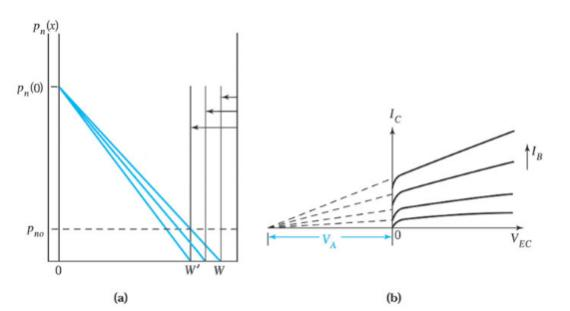
\includegraphics[width=10cm]{figures/ch01/bjt7.jpg}
\caption{Schematic diagram of (a) the Early effect and (b) Early voltage $V_A$} 
\label{fig:bjt7}
\end{figure}

%\section{Field-Effect Transistor}
%\newpage
%\section{JFET}
%PM

\newpage
\section{MOSFET}
\label{sec:mosfet}
The metal–oxide–semiconductor field-effect transistor or \emph{MOSFET} is a transistor based on the field-effect. It has an insulated gate, made of a conductor like a metal or poly-silicon. This terminal is isolated from the rest of the device by a narrow layer of $SiO_2$ which serves as dielectric. The voltage applied at the gate determines the conductivity of the device and hence can control the current between the two other terminals named source and drain. This ability to change conductivity with the amount of applied voltage can be used for amplifying or switching electronic signals. Figure \ref{fig:mosfet1}(a) shows the structure of a MOSFET, while Figure \ref{fig:mosfet1}(c) shows its symbols together with the three terminals.
\subsection{Description and Operation}
Figure \ref{fig:mosfet1}(b) shows the cross-section of an n-channel MOSFET. Source (S) and drain (D) are both $n^+$ contacts and are isolated from each other by the p-type substrate. As the voltage on the gate increases, the holes in the p-type material are expelled and the region below the gate becomes depleted of charge carriers. If the gate voltage increases even further, electrons which are present in the p-type bulk as minority carriers are attracted to the region below the gate. A narrow layer of electrons between source and drain is formed and conduction of electrons between source and drain becomes possible. If the electron density below the gate is equal to the hole concentration in the bulk, inversion has happened and we say that a channel has formed. The gate voltage at which this inversion from p-type to n-type happens, is called the threshold voltage $V_T$.\\
To have a current flow from source to drain, we don't only need a channel but also a positive voltage difference between drain and source. As we increase the voltage at the drain, the current increases, but at the same time the depth of the channel at the drain decreases because $V_{GD} < V_{GS}$. At a certain moment the voltage difference between gate and drain is no longer enough to sustain an n-type channel ($V_{GD} = V_T$). We call this \emph{pinch-off} and say that the transistor is saturated. The current between drain and source no longer increases as the drain voltages increases but remains constant.

\begin{figure}[h!]
\centering
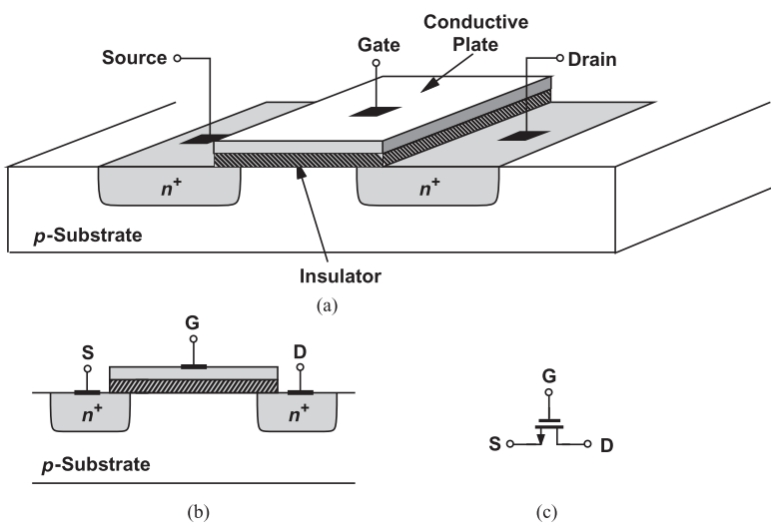
\includegraphics[width=10cm]{figures/ch01/mosfet1b.jpg}
\caption{Schematic diagram of a n-channel MOSFET: (a) structure, (b) side view, (c) symbol} 
\label{fig:mosfet1}
\end{figure}

The dimensions of a MOSFET can become very small; a typical gate oxide thickness $t_{ox}$ is about $15 \AA$ and shrinks with every new generation. The channel length $L$ is typically multiple tens of nanometers.

\subsection{MOS Capacitor}
The region below the gate is a called a MOS capacitor. In integrated circuits, it can store charges and forms the basis building block for charge-coupled devices (CCD). A MOSFET can thus be seen as a MOS capacitor and two pn-junctions placed immediately adjacent to it. We will briefly see how charge builds up in the semiconductor as a voltage is applied to the metal gate.\\
Figure  \ref{fig:moscap} represents a MOS capacitor with the gate on the left and the p-type semiconductor on the right of the oxide. If a negative voltage $V < 0$ is applied to the metal plate of the gate, as in \ref{fig:moscap}(a), positive carriers are attracted to the $SiO_2 - Si$ interface. No current flows in the device, so the Fermi level remains constant. The carrier distribution depends on the difference $E_i - E_F$: $p_p = n_i e^{(E_i - E_F)/kT}$ so the conduction and valence bands at the interface have to bend upward to increase $E_i - E_F$ because $E_F$ is constant. The holes "float" up to the maximum in the valence band and accumulate at the interface.\\
If $V > 0$, as in  \ref{fig:moscap}(b), holes are repelled from the interface and the bands bend up. Initially, all acceptor donors are exposed and a charge layer of depth $W$ is created inside the semiconductor. The induced charge density per unit area is $Q_d = q N_A W$. We call this process \emph{depletion}. If $V$ increases further and the bands bend even more, the intrinsic Fermi level will fall below the true Fermi level as in \ref{fig:moscap}(c) and electrons will swarm to the interface because the exponent in expression $n_p = n_i e^{(E_F - E_i)/kT}$ becomes positive. This process is called \emph{inversion} and is the condition needed to form a channel in a MOSFET. The channel is a highly charged region just right of the interface (see the charge distribution), separated from the p-type semiconductor by a relatively wide depletion region. The voltage where the Fermi levels cross is the threshold voltage $V_T$ and we denote the associated charge $Q_n$.
\begin{figure}[h!]
\centering
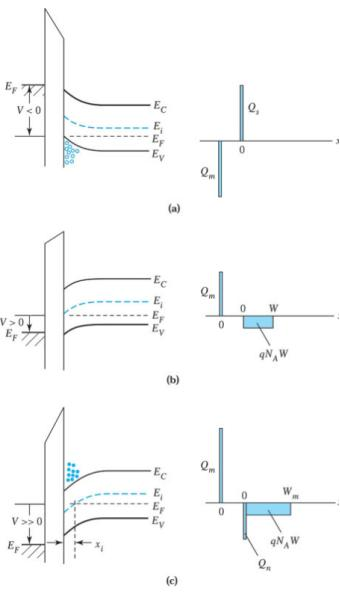
\includegraphics[width=7cm]{figures/ch01/moscap.jpg}
\caption{Band diagrams and charge distribution of a MOS capacitor in (a) accumulation, (b) depletion, and (c) inversion} 
\label{fig:moscap}
\end{figure}

\subsection{I-V characteristic}
\label{sec:MOS_IV}
If $V$ is the applied voltage difference to the plates of a capacitor, and $C$ is the  capacitance, then the  induced charge is $Q = C V$. In the case of the MOSFET of figure \ref{fig:mosfet1}(b), we are only interested in the mobile charges under the gate, namely the electrons $Q_n$ attracted to the interface in figure \ref{fig:moscap}(c), and not the depletion charge $Q_d = q N_A W$. This means that $V = V_{GS} - V_T$ because no mobile charges exist for $V_{GS} < V_T$\footnote{This assumption will be revised in section \ref{sec:subthreshold_conduction}}. If we assume that the MOS capacitor has a gate capacitance $C_{ox}$ per unit area, this relation becomes
$$Q_n = W C_{ox} (V_{GS} - V_T)$$
with $W$ the width of the transistor. Mind that $Q_n$ is a charge density per unit length. As drain and source voltage are not the same, the channel voltage varies along the length of the channel. If we denote the channel potential by $V(x)$, we can rewrite the equation above as:
$$Q_n(x) = W C_{ox} (V_{GS} - V(x) - V_T)$$
where $V(x)$ goes from zero to $V_D$ if the channel is not pinched off (figure \ref{fig:mosfet2}(a)).\\
We know that the current is the charge density times the velocity of the charges: $I_D = Q_n(x) \cdot v$. The current is a drift current as we apply an electric field $\mathcal{E}$ across the channel. Thus:
$$v = -\mu_n \mathcal{E} = \mu_n \frac{dV}{dx}$$
with $\mu_n$ the electron mobility. Substituting this in the expression for $I_D$, we find:
$$I_D = W C_{ox} (V_{GS} - V(x) - V_T) \mu_n \frac{dV(x)}{dx}$$
Multiplying both sides by $dx$ and integrating from $x = 0$ to the channel length  $L$:
$$
 \int_{x=0}^{x=L} I_D dx = \int_{V(x)=0}^{V(x)=V_{DS}} \mu_n C_{ox} W (V_{GS}-V(x)-V_T)dV 
$$
Because $I_D$ is constant along the channel, we can solve both integrals and express $I_D$ as
\begin{equation}
\begin{split}
    I_D = \frac{1}{2} \mu_n C_{ox} \frac{W}{L} [ 2(V_{GS} - V_T) V_{DS} - V_{DS}^2 ]
\end{split}
\end{equation}
This is a parabolic function that reaches a maximum for $V_{DS} = V_{GS} - V_T$:
$$I_{D, max} = \frac{1}{2} \mu_n C_{ox} \frac{W}{L} (V_{GS} - V_T)^2$$
We already established that the condition for saturation is $V_{GD} = V_T$: from this point on, the current will no longer increase as $V_{DS}$ increases because pinch-off has occurred at the drain. Because $V_{DG} = V_{DS} - V_{GS}$ and at pinch-off $V_{DG} = -V_T$, we can rewrite this condition as  $V_{DS} = V_{GS} - V_T$, i.e. at the maximum of the curve, the transistor goes in saturation. This is the situation in figure \ref{fig:mosfet2}(b) and (c). As $V_{DS}$ increases, the pinch-off point $P$ moves closer to the source. The voltage difference in the shrinking channel at $P$ remains $V_{GS} - V_T$. The transistor is in saturation\footnote{Mind that saturation for a MOSFET is not the same concept as saturation for a BJT} and the drain current is - in a first approximation - equal to:
\begin{equation}
    I_{D} = \frac{1}{2} \mu_n C_{ox} \frac{W}{L} (V_{GS} - V_T)^2
    \label{eq:sat_current}
\end{equation}
Note that contrary to the BJT, there is no DC current through the gate.\footnote{A note on notation: we will often use $K$ for the product $\mu_n C_{ox}$.}

\begin{figure}[h!]
\centering
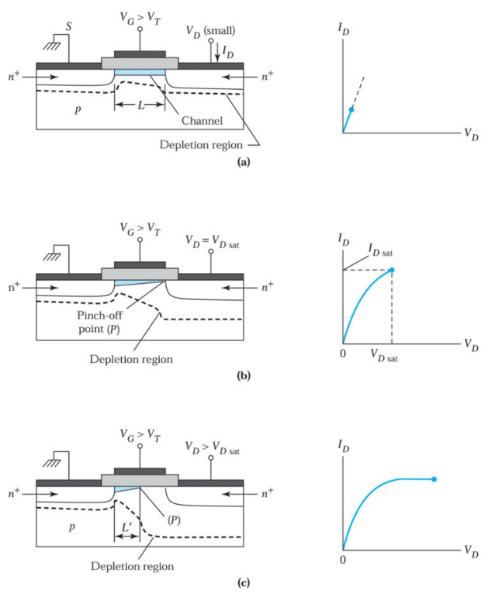
\includegraphics[width=12cm]{figures/ch01/mosfet2.jpg}
\caption{Operations of the MOSFET and output I-V characteristics. (a) Low drain voltage. (b) Onset of saturation. (c) Beyond saturation.} 
\label{fig:mosfet2}
\end{figure}

If $V_{DS}$ is relatively small, we can approximate $I_D$ as:
$$I_D \approx  \mu_n C_{ox} \frac{W}{L} (V_{GS} - V_T) V_{DS}$$
This is the expression of a resistor with value:
$$R_{on} = \frac{1}{\mu_n C_{ox} \frac{W}{L} (V_{GS} - V_T)}$$
We say that the transistor is in the \emph{linear} or \emph{triode} region. Since the resistance is a function of $V_{GS}$, the MOSFET in this region can be seen as a programmable resistance.
%$$I_{D} = \frac{1}{2} \mu_n C_{ox} \frac{W}{L} (V_{GS} - V_T)^2$$

Figure \ref{fig:mosfet3} gives the overall output characteristic of an n-channel MOSFET. Notice how the transition point from linear to saturation depends on $V_{GS}$: for the transistor te be in saturation $V_{DS}$ must be larger than the \emph{overdrive voltage} $V_{ov} = V_{GS} - V_T$, also called the saturation voltage $V_{DS, Sat}$. This is not the case for the BJT, where we used a fixed cutoff $V_{CE,sat}$ with a value of $0.2$ V.

\begin{figure}[h!]
\centering
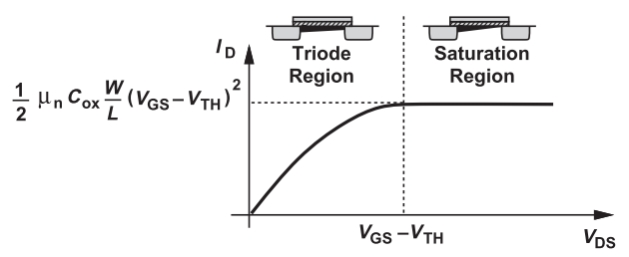
\includegraphics[width=10cm]{figures/ch01/mosfet3.jpg}
\caption{Overall MOSFET $I_D - V_{DS}$ characteristic} 
\label{fig:mosfet3}
\end{figure}
We have studied the n-channel MOSFET or \emph{NMOS}. The study of the p-channel MOSFET or \emph{PMOS} is left as an exercise for the reader.

\subsection{Second Order Effects}
We will discuss several second-order effects that will cause the MOSFET to behave differently than the ideal behavior of figure \ref{fig:mosfet3}.
\subsubsection{Channel-length Modulation}
Notice that in figure \ref{fig:mosfet3}(c) the effective length of the channel decreases as the drain voltage increases (the pinch-off point moves to the left). We established equation \ref{eq:sat_current} with the implicit assumption that $L$ is constant. If however the effective channel length decreases, current $I_D$ will increase with increasing $V_{DS}$ and the I-V characteristic of figure \ref{fig:mosfet3} is not flat. This is similar to the Early effect in the BJT.\\
To model this, we assume that $L$ doesn't change, but do include an explicit dependence on $V_{DS}$ in equation \ref{eq:sat_current}:
\begin{equation}
    I_{D} = \frac{1}{2} \mu_n C_{ox} \frac{W}{L} (V_{GS} - V_T)^2 \; (1 + \lambda V_{DS})
    \label{eq:sat_current2}
\end{equation}
The factor $\lambda$ is the \emph{channel length modulation coefficient}. To decrease $\lambda$, the designer can increase the length of the transistor, because this makes the relative impact of a change in $L$ is smaller.
\subsubsection{Body Effect}
Until now, we have supposed that both the p-type substrate and the n-type source are connected to a common ground. This is however not always the case in real circuits, where the source can be tied to voltages higher than the substrate. Even in that case, the pn-junction between source and substrate is still reversed biased and the device still works properly.\\
However, something does change as the source voltage increases with respect to the bulk: as the source becomes more positive with respect to the substrate, the threshold voltage $V_T$ increases. Called “body effect,” this phenomenon is formulated as
$$V_T = V_{T0} + \gamma (|2\phi_F + V_{SB} - |2\phi_F|)$$
where $V_{SB}$ is the voltage difference between source and  substrate (bulk), $V_{T0}$ the threshold voltage when $V_{SB} = 0$ and $\gamma$ and $\phi_F$ technology-dependent parameters.
\subsubsection{Subthreshold Conduction}
\label{sec:subthreshold_conduction}
We have assumed that the MOSFET turns on abruptly when the gate voltage exceeds the threshold voltage. In practice however, the device turns on gradually and there is already a source-drain current before $V_T$ is reached. This current depends exponentially on $V_{GS}$, similarly as in a BJT. Called the \emph{subthreshold conduction}, this effect has become a critical issue in modern MOS devices.